\section{Applicazione}

L'applicazione principale del progetto è la StreamApp composta principalmente da due Streaming
Query e da un task eseguito periodicamente.

Grazie a Spark Structured Streaming è infatti possibile trattare dati strutturati ottenuti in
real-time da fonti come Apache Kafka similmente a delle tabelle SQL utilizzando strutture chiamate
Dataframe.

\begin{figure}
    \begin{lstlisting}[language=json,firstnumber=1]
    // Schema del json
    val binance_schema = new StructType()
          ...
          .add("a", "string")
          .add("timestamp", "string")
    
    val binance = spark.readStream
        .format("kafka")
        .option("kafka.bootstrap.servers", kafkaBootstrapServers)
        .option("subscribe", pricesTopic)
        .load.select(
        from_json($"value".cast("string"), binance_schema).alias("value"))
        .withColumn("askprice", $"value.a".cast(DoubleType))
        ...
        .withColumn("timestamp",
        ($"value.timestamp".cast(DoubleType)).cast(TimestampType))
        .writeStream
        .foreachBatch {
            (batchDF: DataFrame, batchId: Long) =>
        batchDF.withColumn("processedat",
                current_timestamp())
            .write
            .format("jdbc")
            .option("driver", "org.postgresql.Driver")
            .option("url", jdbcUrl)
            ...
            .save()
        }.start()
    \end{lstlisting}
    \caption{Esempio di Streaming Query}
    \label{streamingquery}
    \end{figure}

Nella Figura \ref{streamingquery} è riportata gran parte della Streaming Query che si occupa
nell'ordine di:
\begin{enumerate}
    \item Configurare le opzioni di connessione a Kafka.
    \item Applicare uno schema corretto ai dati (il corpo dei messaggi Kafka è contenuto nel campo
    value) rinominandoli opportunamente e utilizzando casting al tipo corretto ove necessario.
    \item Aggiungere eventuali informazione ai dati; per esempio viene aggiunto il campo
    "processedat" con il timestamp corrente allo scopo di facilitare la valutazione delle performance.
    \item Scrivere i dati nel database TimescaleDB (attraverso il driver jdbc di postgresql). Questa
    operazione viene svolta attraverso la direttiva foreachBatch in quanto attualmente non è
    possibile scrivere dati da una Streaming Query direttamente in un database, ma è possibile farlo a
    partire da normali Dataframe. Perciò avvalendosi di foreachBatch si può ovviare a questo
    problema aggregando iterativamente i dati ottenuti da una Streaming Query in semplici Dataframe
    il cui contenuto può essere scritto semplicemente in un database.

\end{enumerate}

\subsection{Analisi}

L'analisi effettuata cerca di valutare la positività dei tweets ricevuti (il target è quindi
binario) attraverso modelli allenati utilizzando come target
l'andamento del prezzo di ask di BTCUSDT relativo al minuto di pubblicazione del tweet in modo
che sia positivo ogni tweet seguito da un aumento del prezzo di ask medio. A tale scopo
è stato definito positivo ogni
minuto il cui successivo abbia un prezzo di ask medio superiore e
negativo altrimenti e di conseguenza un tweet è considerabile positivo se pubblicato durante un
"minuto positivo".

In Figura \ref{streamingquery} è illustrato come i dati finanziari contenenti i prezzi di ask
vengono ottenuti e salvati nel database tramite una Streaming Query,
tuttavia la singola Streaming Query non è sufficiente
a calcolare il valore medio del prezzo di ask per minuto; sono infatti necessarie due query: una
per salvare i dati ed una seconda per computare il prezzo medio ogni minuto. Per ovviare a
quest'ultima esigenza StreamApp istanzia un timer che periodicamente esegue le operazioni necessarie
per calcolare il prezzo di ask medio e la polarità di ogni minuto a partire dai
dati salvati nel database per poi scriverne i risultati in una specifica tabella. Il procedimento
è riassunto in Figura \ref{trendpermin}.

\begin{figure}
    \begin{lstlisting}[language=json,firstnumber=1]
val averagePerMin = priceDB
    .groupBy(window($"timestamp", "1 minute"))
    .agg(avg("askprice"))
    ...

val trendPerMin = averagePerMin
    .join(
        averagePerMin
        //renaming column to new_*
        ...
    )
    .filter(expr("timestamp + interval '1 minute' = new_timestamp"))
    .withColumn("asktrend", $"new_avgaskprice" >= $"avgaskprice")
    \end{lstlisting}
    \caption{Calcolo del prezzo di ask medio al minuto}
    \label{trendpermin}
\end{figure}

Infine l'ultima Streaming Query si occupa dei tweets; effettua fondamentalmente le stesse operazioni
dell'altra streaming query eccetto che la fase di aggiunta di informazioni è più complicata in quanto
esegue l'analisi vera e propria per classificare la polarità dei tweets attraverso modelli
precedentemente allenati tramite la TrainApp.

La classificazione risulta essenzialmente una \textit{Sentiment Analysis} supervisionata e sfrutta alcune
funzionalità della libreria MLlib di Spark; implica nell'ordine di:

\begin{enumerate}
    \item Separare l'input in token.
    \item Rimuovere le cosiddette "stop-words".
    \item Eseguire lo "stemming" su ogni token.
    \item Trasformare l'input tramite word embedding in modo da ottenere una rappresentazione
    utilizzabile per allenare un modello di machine learning; è stato utilizzato
    Word2Vec.
    \item Infine fornire la rappresentazione ottenuta tramite Word2Vec come input ad una Regressione
    Logistica, in grado di classificare target binari.
\end{enumerate}

Ognuno di questi step, eccetto lo stemming, utilizza funzioni fornite dalla MLlib di Apache Spark
e per questo motivo si tratta di operazioni scalabili orizzontalmente sui vari nodi del cluster.
Per quanto riguarda lo stemming invece non è stato possibile utilizzare librerie sviluppate
appositamente per l'ultima versione di Spark ma è stato utilizzato Apache OpenNLP, tuttavia
riuscendo ugualmente a rendere l'esecuzione di questo step distribuibile su più nodi.

In Figura \ref{streamapp} è riportato uno schema del funzionamento di StreamApp.

\begin{figure}[h!]
    \centering
    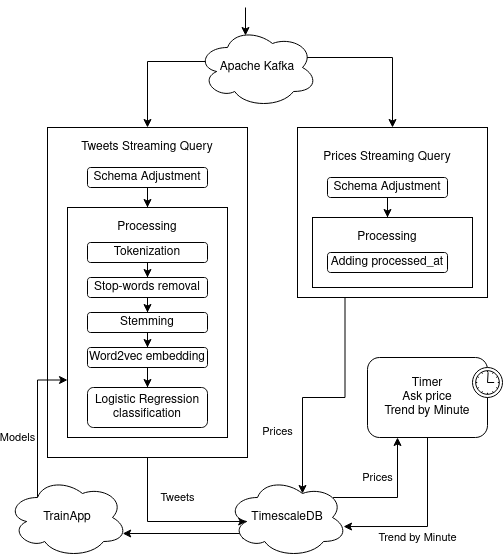
\includegraphics[
		height=10cm,
		keepaspectratio,
    ]{streamapp.png}
    \caption{Schema del funzionamento di StreamApp}
    \label{streamapp}
\end{figure}

\subsection{Training}

Il training dei modelli è svolto per conto della TrainApp: a partire dai tweets
salvati nel database sono stati eseguiti alcuni degli stessi passaggi necessari per
l'analisi in streaming, quali:

\begin{enumerate}
    \item Tokenizzazione.
    \item Rimozione delle stop-words.
    \item Stemming.
\end{enumerate}

Per poi utilizzare i token rimasti per il training del modello Word2Vec, ed in seguito
impiegare la
rappresentazione Word2Vec, come input, insieme all'andamento del prezzo di ask al minuto,
come target,
per allenare il modello di Regressione logistica.

\subsection{Performance del modello}

La TrainApp stessa prima della creazione del modello finale utilizzando la totalità dei dati
ne esegue una validazione dividendo il dataset in trainset e testset e computando il valore AUC
(Area Under ROC).
Purtroppo i risultati ottenuti non sono dei migliori: i valori di AUC sono intorno a 0.5, cioè
le performance sono paragonabili a una scelta random.

Ciò può significare che il contenuto dei tweets generalmente non è correlato all'andamento
del prezzo di ask.
Potrebbe perciò rivelarsi utile un
filtraggio manuale di un insieme ristretto di tweets in modo da selezionare solo quelli rilevanti.

In aggiunta un'ulteriore operazione manuale di etichettatura potrebbe chiarire se l'andamento
dei prezzi sia un parametro adeguato a definire la polarità dei tweets.